% ---------------------------------------------------------------------------
% Savant: methods, results, and a discussion outline.
%
% Every number in this file is transcribed from a file in the repository. The
% source is named in a comment beside each table so that any figure can be
% traced back and re-checked after a re-run. Figures are produced by
% report/make_figures.py and written to report/figures/.
%
% Compile with: pdflatex savant_methods_results.tex  (twice, for references)
% ---------------------------------------------------------------------------
\documentclass[11pt]{article}

\usepackage[T1]{fontenc}
\usepackage[utf8]{inputenc}
\usepackage[margin=1in]{geometry}
\usepackage{graphicx}
\usepackage{booktabs}
\usepackage{amsmath}
\usepackage{amssymb}
\usepackage{caption}
\usepackage{float}
\usepackage{xcolor}
\usepackage{enumitem}
\usepackage[hidelinks]{hyperref}

\graphicspath{{figures/}}
\captionsetup{font=small, labelfont=bf}
\setlist[itemize]{itemsep=2pt, topsep=4pt}
\setlist[enumerate]{itemsep=2pt, topsep=4pt}

\newcommand{\pkd}{\ensuremath{\mathrm{pK_d}}}

\title{Savant: structure-free protein--ligand affinity prediction on CPU\\
\large Methods, results, and discussion outline}
\author{Sayal Guirales-Medrano}
\date{\today}

\begin{document}
\maketitle

\begin{abstract}
\noindent
Predicting the affinity of a small molecule for a protein target is the central
quantitative problem of early drug discovery. Current leading methods co-fold
the protein--ligand complex before scoring it, which is accurate but requires a
graphics processing unit (GPU) and substantial time per pair. We developed
Savant, a model that predicts binding affinity (\pkd) from an amino acid
sequence and a ligand Simplified Molecular-Input Line-Entry System (SMILES)
string alone, without an experimental or predicted structure, without docking,
and without a GPU. We built the model in 2 phases. We first trained a
structure-based model on 47,619 protein--ligand complexes refined with
HADDOCK3, and we measured how its accuracy scales with the number of docked
complexes. We then trained a structure-free model on the full corpus of 1.9
million measured pairs. To evaluate the model, we assembled a benchmark of 500
protein--ligand pairs across 20 targets, restricted to measurements published
in 2025 or later and to ligands dissimilar to anything in training, and we
compared Savant against Boltz-2, PRODIGY-LIG, PLAPT, per-target quantitative
structure--activity relationship (QSAR) models, and a Tanimoto nearest-neighbor
predictor. We show that Savant's accuracy is concentrated in one regime. Savant
achieves the highest mean within-target rank correlation of any method tested
($\rho = 0.278$ across 20 targets, compared to 0.228 for Boltz-2), and it
outperforms models fitted on each target's own prior compounds. Conversely,
Savant does not rank targets against one another for a fixed ligand, and it
does not produce a calibrated absolute affinity. We conclude that the method is
suited to screening one protein against many ligands.
\end{abstract}

\tableofcontents

% ===========================================================================
\section{Methods}
% ===========================================================================

\subsection{Data acquisition and preparation}

We sourced training data from the \texttt{jglaser/binding\_affinity}
collection, which was assembled from BindingDB, PDBbind-CN, BioLIP, and
BindingMOAD. The collection comprises 1.9 million protein sequence and ligand
SMILES pairs with measured affinities. We expressed all affinities as
\[
  \pkd = -\log_{10} K_d \quad (K_d \text{ in } \mathrm{M}).
\]

Two properties of this label govern the interpretation of every result reported
below. Both are properties of the measurement rather than of any model.

First, the label pools assay types. The released file provides a single
affinity column and does not provide a \texttt{standard\_type} field.
Dissociation constants ($K_d$), inhibition constants ($K_i$), and half-maximal
inhibitory concentrations (IC$_{50}$) are therefore mixed and cannot be
separated after the fact. IC$_{50}$ in particular depends on assay conditions
that the file does not record, so a portion of the label variance is not a
function of the protein--ligand pair at all.

Second, the label is noisy, and we were able to quantify the noise. We found
that 11.9\% of unique sequence and SMILES pairs appear more than once in the
corpus. These replicates disagree by a pooled standard deviation of 0.81 \pkd,
meaning that identical inputs carry different recorded answers. A model that
recovered the true value exactly would still score a root mean squared error
(RMSE) of approximately 0.81 against single measurements. We therefore read
every error figure in this study against that floor rather than against zero.

\subsection{Phase 1: structure-based modeling of docked complexes}
\label{sec:phase1}

The first Savant model consumed physically docked complexes. For 47,619
protein--ligand pairs, we generated and refined structures using HADDOCK3 with
a \texttt{[topoaa]} topology generation stage followed by an \texttt{[emref]}
energy minimization stage. From the resulting Critical Assessment of PRedicted
Interactions (CAPRI) table we read 6 energy terms: \texttt{score},
\texttt{total}, \texttt{vdw}, \texttt{elec}, \texttt{desolv}, and \texttt{bsa}.
We computed a seventh, geometric term directly from the pose, defined as the
count of protein residues having any atom within 6.0 \AA{} of any ligand atom.

We concatenated these 7 terms with features derived from the sequence and the
SMILES string alone:

\begin{itemize}
  \item a ChemBERTa-77M-MLM embedding of the ligand (384 dimensions),
  \item an ESM2-8M embedding of the protein (320 dimensions),
  \item RDKit physicochemical descriptors computed on the hydrogen-added
        molecule (11 columns), together with the surviving RDKit descriptor set
        (212 columns, after dropping columns that were constant across the
        training data),
  \item an Extended Connectivity Fingerprint of diameter 4 (ECFP4) count
        fingerprint (1,024 dimensions),
  \item amino acid composition and chain length (21 columns).
\end{itemize}

We mean-pooled all embeddings over the last hidden state with padding masked
out. We defined a structure-free variant of the same model that is identical
except that the HADDOCK3 block is absent, giving 1,972 features against 1,979.
The difference between the 2 variants therefore isolates the contribution of
the docked structure.

We fitted all models with XGBoost under 3 held-out regimes: protein-grouped, in
which no protein is shared between the training and test sets; ligand-grouped;
and both-disjoint. Rows from different regimes are not comparable to one
another, because each regime defines its own test set. The comparison that
carries meaning is structure-based against structure-free within a single
regime.

\subsection{Learning-curve experiment}
\label{sec:curve-methods}

The Phase 1 model used 47,619 docked complexes, which is 2.6\% of the available
pairs. Producing the remainder would require substantial compute. To determine
whether that compute would be worthwhile, we measured the shape of the learning
curve directly.

We fixed a single protein-grouped test set at the outset and did not modify it
thereafter. We then trained models on increasing fractions of the remaining
pairs (0.1, 0.2, 0.3, 0.4, 0.6, 0.8, and 1.0), with and without the HADDOCK3
block at every size, and we repeated each size over independent subsamples so
that we could report the spread across repeats alongside the mean. Because the
test set is fixed, points on the curve are comparable to one another, which
would not be the case if each size drew its own split. This experiment is
implemented in \texttt{ML\_model/learning\_curve\_structure\_based.py}.

\subsection{Phase 2: structure-free modeling of the full dataset}
\label{sec:phase2}

Docking 1.9 million complexes was not feasible within this project. We
therefore removed the structure entirely and instead acquired accuracy from
data. We retained every feature derivable from the sequence and the SMILES
string, and we trained on the full corpus. This is the production model, and we
refer to it hereafter simply as Savant.

\begin{table}[H]
\centering
\caption{Feature layout of the production model, comprising 2,935 features.
Block order is load-bearing and must match the order used in training.}
\label{tab:blocks}
\begin{tabular}{llr}
\toprule
Block & Source & Width \\
\midrule
ChemBERTa-77M ligand embedding      & SMILES   & 384 \\
RDKit named descriptors             & SMILES   & 226 \\
ECFP4 count fingerprint             & SMILES   & 1024 \\
ESM2-650M protein embedding         & sequence & 1280 \\
Amino acid composition and length   & sequence & 21 \\
\midrule
\multicolumn{2}{l}{Total}                      & 2935 \\
\bottomrule
\end{tabular}
\end{table}

We also trained a second variant in which ESM2-650M is replaced by the 80-fold
smaller ESM2-8M (320 dimensions, giving 1,975 features in total). We trained
this variant on the same rows, using the same split and the same
hyperparameters, so that any difference between the 2 variants is attributable
to the protein representation alone.

We trained with XGBoost under squared-error loss and a protein-grouped split.
The inner split used for early stopping holds out the same grouping key as the
outer split. A random inner split would allow the model to tune against
proteins on which it is subsequently tested, which inflates the reported score
without improving the model. We averaged replicate measurements of the same
sequence and SMILES pair into a single label before fitting, so that a
frequently re-measured pair does not receive proportionally more weight than a
singly measured one.

To prevent the benchmark from measuring memorization, we removed benchmark
ligands from the training set before fitting any production model.
Specifically, we dropped every training ligand within an ECFP4 Tanimoto
similarity of 0.50 of any benchmark ligand.

Earlier revisions of the model trained a separate XGBoost classifier alongside
the regressor. Within the single revision that carries both heads, the
classifier gained 0.012 in area under the receiver operating characteristic
curve (ROC AUC) over thresholding the regressor at the \pkd{} 6 cut (0.678
against 0.666) and lost 0.010 at the \pkd{} 7 cut (0.561 against 0.571). We
found no consistent gain, and the classifier consumed half of the training
budget. The production model therefore ships with the regressor only, and we
make binder calls by thresholding the predicted \pkd. This has the additional
advantage that the threshold is selected at inference time rather than fixed
during training.

\subsection{Benchmark construction}
\label{sec:bench-methods}

To evaluate the production model we assembled a benchmark of 500
protein--ligand pairs across 20 targets. We constructed the set to be difficult
in 3 specific respects.

\begin{itemize}
  \item \textbf{Ligand novelty.} Every benchmark ligand falls below an ECFP4
        Tanimoto similarity of 0.50 to anything in Savant's training set. The
        realized maximum is 0.494.
  \item \textbf{Temporal separation.} Every measurement dates from 2025 or
        later and is absent from ChEMBL v34 (April 2024), the release most
        plausibly contained within Boltz-2's training window.
  \item \textbf{Assay filtering.} We retained $K_d$ and $K_i$ measurements only,
        at a ChEMBL confidence score of 8 or greater.
\end{itemize}

We deliberately did not require novel proteins. The training corpus covers
essentially every well-measured target, so a novel-protein requirement would
have left only sparsely characterized targets, for which the ground truth is
itself unreliable. All 20 benchmark targets therefore appear in training with
other ligands. This benchmark measures the ranking of novel chemistry against
an established target, which is the realistic screening scenario, and results
obtained from it must not be described as zero-shot with respect to the target.

The temporal filter protects every method equally, because no method trained
before 2025 can have seen these measurements. Both Boltz-2 and PLAPT predate
the cutoff. The ligand similarity filter, however, does not transfer between
methods, and the direction in which this cuts is worth stating explicitly. We
applied the near-neighbor removal to Savant's training set only. The comparison
methods were trained by other groups on other corpora and may well retain close
analogues of these benchmark ligands. Savant is therefore held to a stricter
novelty standard than the methods against which we compare it, and any
advantage it shows is measured under that handicap.

We additionally performed a difference-in-differences audit on the predecessor
1,000-pair benchmark to test whether Boltz-2's pooled advantage is attributable
to having seen the pairs. The estimated effect was 0.111 Pearson $r$ (95\%
confidence interval $-0.090$ to 0.299, one-sided $P = 0.14$), which we do not
regard as evidence of memorization. We report this audit as context, because it
was performed on the earlier benchmark rather than on the 500-pair set.

\subsection{Comparison methods}

\begin{table}[H]
\centering
\caption{The methods compared, and the input each requires at inference time.}
\label{tab:tools}
\small
\begin{tabular}{p{0.19\textwidth}p{0.48\textwidth}p{0.21\textwidth}}
\toprule
Method & Description & Requires \\
\midrule
\textbf{Savant} & This work. Gradient-boosted trees over protein and ligand
language-model embeddings, RDKit descriptors, and a fingerprint &
sequence and SMILES, CPU \\
\textbf{Boltz-2} & Co-folds the protein--ligand complex with a diffusion
model, then predicts affinity from the predicted structure &
sequence and SMILES, GPU \\
\textbf{PLAPT} & The closest published peer. ProtBERT and ChemBERTa
embeddings passed to a small neural head, also structure-free &
sequence and SMILES \\
\textbf{PRODIGY-LIG} & Physics-based rescoring. A linear model over atomic
contact counts in an existing complex & a 3-D complex \\
\textbf{QSAR (per-target)} & A separate model fitted on one target's own
previously measured compounds & prior data for that target \\
\textbf{Tanimoto $k$-NN} & Predicts from the chemically most similar known
actives for that target & prior data for that target \\
\bottomrule
\end{tabular}
\end{table}

The final 2 methods warrant description, because they are the baselines a
computational chemist would ordinarily construct and they are not
general-purpose tools. The per-target QSAR baseline fits a separate model for
each benchmark target using only that target's previously measured compounds.
This is the classical quantitative structure--activity relationship approach,
which knows one protein well and knows nothing else. The Tanimoto $k$-NN
baseline fits nothing at all. For a query ligand it retrieves the most
structurally similar compounds previously measured against the same target,
ranked by ECFP4 Tanimoto similarity, and predicts their affinity. It represents
the assumption that similar molecules bind similarly, and it is the appropriate
floor for a benchmark built from novel chemistry, because a benchmark on which
similarity search already succeeds would not be testing generalization.

We also report a constant-mean predictor, which returns the benchmark average
for every pair. It is not a competing method. We include it in every error
table because it establishes whether a given RMSE figure carries information.

\subsection{Evaluation design}
\label{sec:eval-methods}

A single pooled correlation computed over all 500 pairs conflates 2 abilities
that serve different purposes and that a model can possess independently. Let
$\hat{y}$ denote the prediction, $y$ the measurement, and $\bar{\;\cdot\;}_t$ a
mean taken within target $t$. We define:

\begin{itemize}
  \item \textbf{Between-target} correlation,
        $\mathrm{corr}(\bar{\hat{y}}_t,\, \bar{y}_t)$ computed over targets,
        which measures which protein binds more tightly;
  \item \textbf{Within-target} correlation,
        $\mathrm{corr}(\hat{y} - \bar{\hat{y}}_t,\, y - \bar{y}_t)$, which
        measures which ligand binds more tightly for a given target.
\end{itemize}

Pooled correlation is a blend of the 2, weighted by the proportion of the
benchmark's variance that lies between targets rather than within them. That
weighting is a property of the benchmark and not of any model, which is why we
report the decomposition alongside the pooled figure rather than in place of
it.

Our evaluation comprises 6 tests, which we describe below and report in
Section 2:

\begin{description}[leftmargin=1.6em, style=nextline]
  \item[Test A, pooled accuracy and its decomposition.] Pearson $r$, Spearman
    $\rho$, RMSE, mean absolute error, bias, coefficient of determination
    ($R^2$), and the ratio of predicted to true standard deviation, computed
    over all pairs, together with the between-target and within-target split
    defined above.
  \item[Test B, one protein against many ligands.] Spearman $\rho$ computed
    within each of the 20 targets and averaged. This corresponds to the
    lead-optimization task.
  \item[Test C, one ligand against many proteins.] For the 26 ligands measured
    against more than one target, Spearman $\rho$ computed across targets.
  \item[Test D and Test E, taxonomy.] Within-target $\rho$ stratified by
    protein family and by ligand chemotype, where chemotypes were assigned
    using RDKit SMARTS classes.
  \item[Test F, comparison against models fitted on the target itself.] Savant
    paired against the per-target QSAR and Tanimoto $k$-NN baselines on the 18
    targets for which sufficient prior data exists to fit a local model.
\end{description}

\subsection{Statistical analysis}

We computed all paired comparisons as cluster-resampled bootstraps. We
resampled targets in Test B and Test F, so that the resulting interval reflects
uncertainty over the units actually sampled rather than over individual pairs.
We report Wilcoxon signed-rank and sign tests alongside each bootstrap. All
confidence intervals are 95\%, and we report a point estimate whose interval
spans zero as parity, irrespective of the sign of the estimate.

\subsection{Runtime measurement}

We measured runtime on CPU, with the protein encoder forced onto CPU
explicitly, because the presence of a visible GPU otherwise alters the
measurement even when the GPU is not intended to be used. We measured 3
quantities separately, because they scale differently: the one-off cost of
embedding a protein, the marginal cost of one additional ligand scored against
an already-embedded protein, and the total for a realistic mixed workload. We
did not take a head-to-head wall-clock measurement of Boltz-2. The runtime
comparison reported below is therefore structural, describing the work each
method must perform per pair, and is not a measured speedup ratio.

% ===========================================================================
\section{Results}
% ===========================================================================

\subsection{Docked structural terms improve prediction across all splits}

Table \ref{tab:phase1} shows the held-out performance of the Phase 1 models.

\begin{table}[H]
\centering
\caption{Phase 1 held-out performance. Rows are not comparable across splits,
because each split defines its own test set. Data source:
\texttt{ML\_model/models\_structure\_free/results.csv}.}
\label{tab:phase1}
\begin{tabular}{llrrrrr}
\toprule
Features & Split & $n$ test & $R^2$ & Pearson $r$ & RMSE & ROC AUC \\
\midrule
structure-free  & protein-grouped & 9116  & 0.400 & 0.633 & 1.163 & 0.799 \\
structure-free  & ligand-grouped  & 10998 & 0.440 & 0.667 & 1.123 & 0.805 \\
structure-free  & both-disjoint   & 2291  & 0.355 & 0.599 & 1.261 & 0.774 \\
structure-based & protein-grouped & 9116  & 0.451 & 0.673 & 1.112 & 0.812 \\
structure-based & ligand-grouped  & 10998 & 0.491 & 0.704 & 1.071 & 0.811 \\
structure-based & both-disjoint   & 2291  & 0.385 & 0.623 & 1.232 & 0.785 \\
\bottomrule
\end{tabular}
\end{table}

Under the protein-grouped split, the docked model reached $R^2 = 0.451$,
compared to $R^2 = 0.400$ for the identical model with the HADDOCK3 block
removed. We observed this advantage consistently across all 3 splits. The
docking terms were worth approximately 0.05 in $R^2$ and 0.035 in Pearson $r$.

\subsection{Performance continues to rise with additional docked complexes}
\label{sec:curve-results}

To determine whether producing additional docked complexes would improve the
model further, we measured the learning curve described in Section
\ref{sec:curve-methods}. Figure \ref{fig:curve} shows the result, and Table
\ref{tab:curve} lists the underlying values.

\begin{figure}[H]
\centering
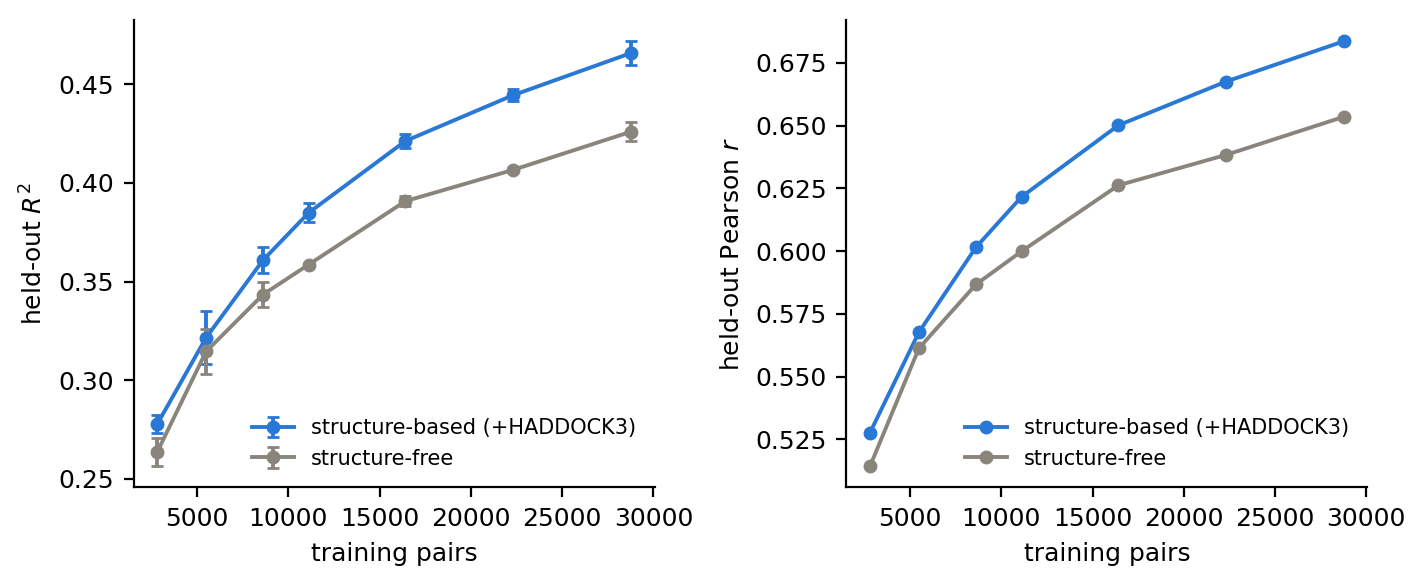
\includegraphics[width=\textwidth]{fig_learning_curve.png}
\caption{Learning curve computed on a fixed protein-grouped test set, with and
without the HADDOCK3 block at every training size. The left panel shows the
coefficient of determination and the right panel shows the Pearson correlation.
Error bars show the spread across repeated subsamples of the same size. Data
source: \texttt{ML\_model/work\_curve/learning\_curve\_summary.csv}.}
\label{fig:curve}
\end{figure}

\begin{table}[H]
\centering
\caption{Learning-curve summary. $R^2_{\mathrm{sd}}$ is the spread across
repeated subsamples drawn at the same size.}
\label{tab:curve}
\small
\begin{tabular}{lrrrrrr}
\toprule
Features & Fraction & $n$ train & $n$ proteins & $R^2$ & $R^2_{\mathrm{sd}}$ & Pearson $r$ \\
\midrule
structure-based & 0.1 & 2{,}810  & 1{,}148 & 0.278 & 0.005 & 0.528 \\
structure-based & 0.2 & 5{,}489  & 2{,}009 & 0.322 & 0.014 & 0.568 \\
structure-based & 0.3 & 8{,}612  & 2{,}771 & 0.361 & 0.007 & 0.602 \\
structure-based & 0.4 & 11{,}111 & 3{,}497 & 0.385 & 0.005 & 0.622 \\
structure-based & 0.6 & 16{,}415 & 4{,}810 & 0.421 & 0.004 & 0.650 \\
structure-based & 0.8 & 22{,}302 & 6{,}033 & 0.445 & 0.003 & 0.668 \\
structure-based & 1.0 & 28{,}767 & 7{,}168 & 0.466 & 0.006 & 0.684 \\
\midrule
structure-free  & 0.1 & 2{,}810  & 1{,}148 & 0.264 & 0.007 & 0.514 \\
structure-free  & 0.2 & 5{,}489  & 2{,}009 & 0.315 & 0.012 & 0.561 \\
structure-free  & 0.3 & 8{,}612  & 2{,}771 & 0.343 & 0.006 & 0.587 \\
structure-free  & 0.4 & 11{,}111 & 3{,}497 & 0.359 & 0.001 & 0.600 \\
structure-free  & 0.6 & 16{,}415 & 4{,}810 & 0.391 & 0.002 & 0.626 \\
structure-free  & 0.8 & 22{,}302 & 6{,}033 & 0.407 & 0.001 & 0.638 \\
structure-free  & 1.0 & 28{,}767 & 7{,}168 & 0.426 & 0.005 & 0.654 \\
\bottomrule
\end{tabular}
\end{table}

Two quantities emerge from this experiment. First, the curve has not flattened.
Over the final segment, the docked model moved from $R^2 = 0.445$ at 22,302
pairs to $R^2 = 0.466$ at 28,767 pairs, which corresponds to a slope of 0.058
in $R^2$ per doubling of the training data. We observed no sign of saturation
at the largest size reached. This result indicates that docking additional
complexes would continue to improve the model, and the slope provides an
approximate budget for how much compute purchases how much accuracy.

Second, the structural contribution is modest and does not vary with scale.
Averaged over all training sizes, the HADDOCK3 block is worth 0.025 in $R^2$,
and in Fig. \ref{fig:curve} we see that the gap between the 2 series neither
closes nor widens materially as the training set grows.

Both readings extrapolate beyond the measured range, and their magnitude should
not be quoted at 1.9 million pairs. What the curve establishes is the direction
and the approximate rate, not the value at the full corpus. These results
motivated the transition described in Section \ref{sec:phase2}. A gain of 0.025
in $R^2$ that costs minutes of docking per complex compares unfavorably against
a gain of 0.058 in $R^2$ per doubling that costs only additional rows,
particularly when approximately 40 times more rows were already available and
undocked.

\subsection{Benchmark composition}

\begin{table}[H]
\centering
\caption{Composition of the 500-pair benchmark. Data source:
\texttt{ML\_model/benchmark/eval/output/bench\_scored.csv}.}
\label{tab:bench}
\begin{tabular}{lr}
\toprule
Pairs                              & 500 \\
Targets                            & 20 \\
Distinct ligand skeletons          & 373 \\
\pkd{} mean                        & 7.296 \\
\pkd{} standard deviation          & 1.274 \\
Maximum ECFP4 Tanimoto to training & 0.494 \\
\bottomrule
\end{tabular}
\end{table}

The label spread of 1.274 \pkd{} is the value against which every RMSE reported
below should be judged, because it is precisely the RMSE achieved by predicting
the benchmark mean for every pair.

\subsection{No method predicts absolute affinity better than a constant}
\label{sec:pooled}

Table \ref{tab:pooled} reports pooled accuracy over all 500 pairs.

\begin{table}[H]
\centering
\caption{Accuracy pooled over all 500 pairs, ignoring which target each pair
belongs to. Spread is the ratio of predicted to true standard deviation, for
which a value of 1.0 would indicate that the predictions are as dispersed as
the measurements. Data source: \texttt{bench\_A\_pooled.csv}.}
\label{tab:pooled}
\begin{tabular}{lrrrrrr}
\toprule
Method & $n$ & Pearson $r$ & Spearman $\rho$ & RMSE & $R^2$ & Spread \\
\midrule
Savant             & 500 & 0.227 & 0.147 & 1.353 & $-0.129$ & 0.425 \\
Boltz-2            & 496 & 0.412 & 0.393 & 1.388 & $-0.193$ & 0.750 \\
PLAPT              & 500 & 0.021 & $-0.032$ & 1.827 & $-1.060$ & 0.824 \\
PRODIGY-LIG        & 496 & 0.333 & 0.340 & 1.537 & $-0.461$ & 1.087 \\
QSAR (per-target)  & 458 & 0.089 & 0.050 & 1.733 & $-0.797$ & 0.663 \\
Tanimoto $k$-NN    & 458 & 0.102 & 0.066 & 1.679 & $-0.688$ & 0.823 \\
\midrule
Constant baseline  & 500 & ---   & ---   & 1.273 & 0.000 & 0.000 \\
\bottomrule
\end{tabular}
\end{table}

Two findings follow from this table, and both concern the benchmark rather than
any individual method.

First, no method outperformed the constant baseline on RMSE. Savant's RMSE of
1.353 is the lowest of any method tested, and is lower than Boltz-2's 1.388,
but it remains higher than the 1.273 obtained by predicting 7.296 for every
pair. Every $R^2$ value in the table is negative. We therefore report no
absolute-error claim for any method evaluated on this benchmark.

Second, Savant's pooled correlation of $r = 0.227$ trails both Boltz-2 (0.412)
and PRODIGY-LIG (0.333). The decomposition presented in Section
\ref{sec:decomp} identifies the source of that deficit, which is not the source
the pooled figure suggests.

In Fig. \ref{fig:spread} we see that Savant produces the most compressed
predictions of any method tested, with a spread ratio of 0.425. Squared-error
training against a noisy label shrinks predictions toward the mean, which
protects RMSE and degrades absolute calibration while leaving the rank order
intact.

\begin{figure}[H]
\centering
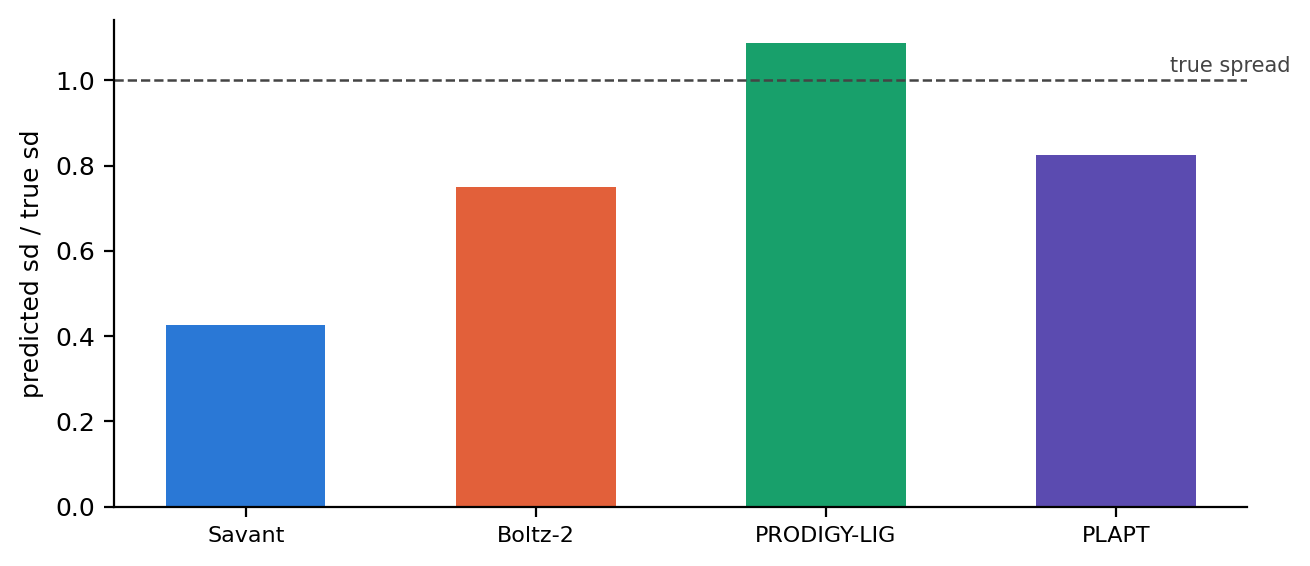
\includegraphics[width=0.85\textwidth]{fig_spread.png}
\caption{Ratio of predicted to true standard deviation for each method. The
dashed line marks the true spread of the benchmark labels. Values below 1.0
indicate predictions that are less dispersed than the measurements.}
\label{fig:spread}
\end{figure}

\subsection{Decomposition reveals that Savant's accuracy is within-target}
\label{sec:decomp}

To identify the source of Savant's pooled deficit, we decomposed the pooled
correlation into its between-target and within-target components as defined in
Section \ref{sec:eval-methods}. Table \ref{tab:decomp} reports the result and
Fig. \ref{fig:decomp} displays it.

\begin{table}[H]
\centering
\caption{Between-target $r$ correlates predicted target means against measured
target means, and corresponds to determining which protein binds more tightly.
Within-target $r$ centers both quantities on the target mean beforehand, and
corresponds to determining which ligand binds more tightly for a given target.
Data source: \texttt{bench\_A\_decomposition.csv}.}
\label{tab:decomp}
\begin{tabular}{lrrr}
\toprule
Method & Between-target $r$ & Within-target $r$ & Pooled $r$ \\
\midrule
Savant            & 0.100 & \textbf{0.436} & 0.227 \\
Boltz-2           & 0.351 & 0.386 & 0.412 \\
PLAPT             & $-0.225$ & 0.208 & 0.021 \\
PRODIGY-LIG       & 0.295 & 0.237 & 0.333 \\
QSAR (per-target) & 0.124 & 0.155 & 0.089 \\
Tanimoto $k$-NN   & 0.135 & 0.066 & 0.102 \\
\bottomrule
\end{tabular}
\end{table}

\begin{figure}[H]
\centering
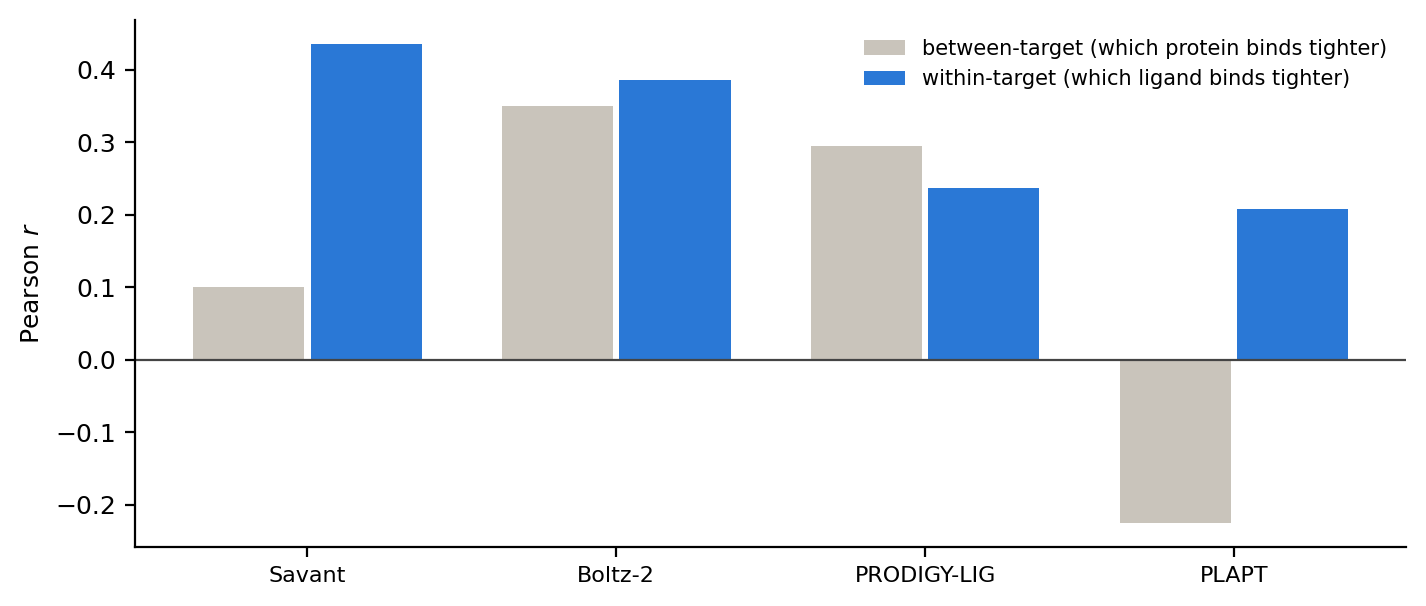
\includegraphics[width=\textwidth]{fig_decomposition.png}
\caption{The 2 abilities separated. Gray bars show between-target correlation
and blue bars show within-target correlation. Savant achieves the highest
within-target correlation of any method tested and nearly the lowest
between-target correlation, whereas Boltz-2 is balanced across the 2. The
pooled figures in Table \ref{tab:pooled} are a weighted blend of these bars,
and the weighting is a property of the benchmark.}
\label{fig:decomp}
\end{figure}

This is the central result of the evaluation. Savant's within-target
correlation of 0.436 is the highest of any method tested and exceeds Boltz-2's
0.386. Conversely, Savant's between-target correlation of 0.100 is close to
zero and far below Boltz-2's 0.351. The pooled deficit reported in Table
\ref{tab:pooled} is therefore attributable entirely to the between-target
component, and on the within-target component Savant leads. These findings
indicate that Savant ranks compounds against a given target at least as well as
a method that folds every complex on a GPU, and that it does not reliably
determine which of 2 proteins binds more tightly.

\subsection{Savant ranks compounds within a target as well as Boltz-2}
\label{sec:within}

To evaluate the lead-optimization task directly, we computed Spearman $\rho$
within each of the 20 benchmark targets and averaged across them. Table
\ref{tab:testb} reports the result.

\begin{table}[H]
\centering
\caption{Within-target Spearman $\rho$, computed within each target and
averaged across targets. The final column counts targets for which $\rho > 0$.
Data source: \texttt{bench\_B\_summary.csv}.}
\label{tab:testb}
\begin{tabular}{lrrrr}
\toprule
Method & Targets & Mean $\rho$ & Median $\rho$ & Positive \\
\midrule
Savant            & 20 & \textbf{0.278} & 0.278 & 16/20 \\
PRODIGY-LIG       & 20 & 0.233 & 0.196 & 15/20 \\
Boltz-2           & 20 & 0.228 & 0.242 & 15/20 \\
QSAR (per-target) & 18 & 0.127 & 0.226 & 12/18 \\
PLAPT             & 20 & 0.067 & 0.111 & 12/20 \\
Tanimoto $k$-NN   & 18 & 0.031 & 0.002 & 9/18 \\
\bottomrule
\end{tabular}
\end{table}

Savant achieved the highest mean within-target Spearman $\rho$ of any method
tested, and produced a positive correlation on 16 of the 20 targets. To
determine whether this advantage is statistically resolvable, we paired each
method against Boltz-2 and resampled targets. Table \ref{tab:testb-paired}
reports the paired comparison.

\begin{table}[H]
\centering
\caption{Each method paired against Boltz-2, with targets resampled by cluster
bootstrap. A confidence interval spanning zero indicates parity, irrespective
of the sign of the point estimate. Data source: \texttt{bench\_B\_vs\_ref.csv}.}
\label{tab:testb-paired}
\begin{tabular}{lrrrr}
\toprule
Method & Mean difference & 95\% CI & Wins & Wilcoxon $P$ \\
\midrule
Savant            & $+0.050$ & $-0.059$ to $+0.159$ & 9/20 & 0.65 \\
PRODIGY-LIG       & $+0.005$ & $-0.144$ to $+0.176$ & 9/20 & 0.87 \\
PLAPT             & $-0.161$ & $-0.305$ to $-0.019$ & 8/20 & 0.07 \\
\bottomrule
\end{tabular}
\end{table}

Savant's point estimate is the highest of any method, but the paired confidence
interval against Boltz-2 spans zero. We therefore report parity with Boltz-2
rather than a demonstrated advantage. Twenty targets do not provide sufficient
resolution to establish a difference of 0.050 in mean $\rho$. What these results
do establish is that a CPU-only, structure-free method matches a GPU co-folding
method on the within-target ranking task, and that it clearly exceeds PLAPT,
per-target QSAR, and similarity search.

In Fig. \ref{fig:within} we see that the 2 methods disagree substantially on
individual targets in both directions, which accounts for the width of the
paired interval despite the similarity of the means.

\begin{figure}[H]
\centering
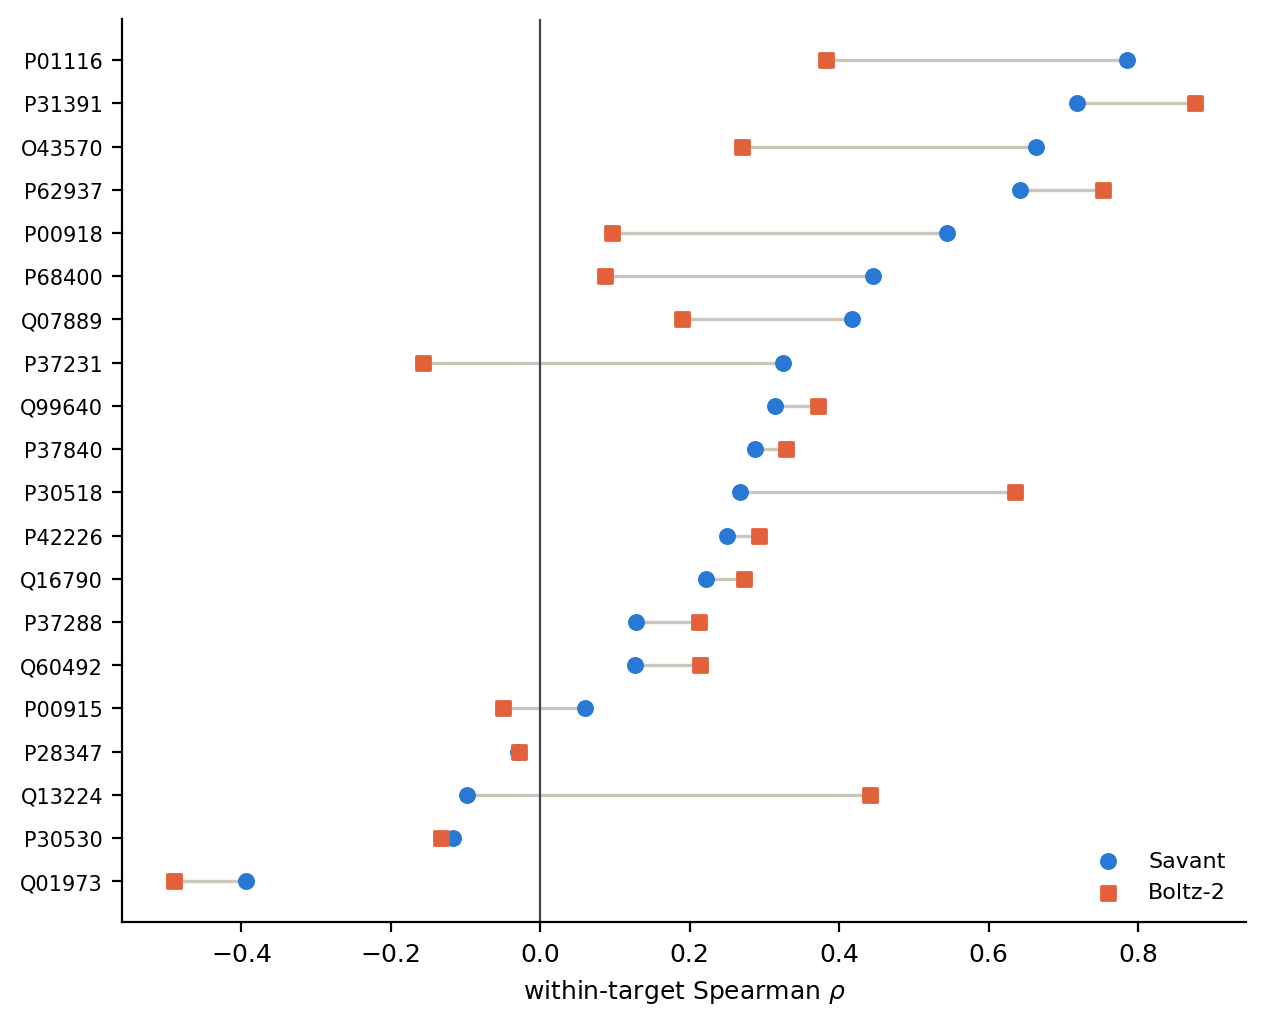
\includegraphics[width=0.78\textwidth]{fig_within_target.png}
\caption{Per-target within-target Spearman $\rho$ for Savant (blue circles) and
Boltz-2 (orange squares), with one row per benchmark target, sorted by Savant.
Savant leads on P01116 (KRAS) and P00918 (carbonic anhydrase II), whereas
Boltz-2 leads on Q13224 (NMDA receptor subunit GluN2B) and P30518 (vasopressin
V2 receptor). Data source: \texttt{bench\_B\_per\_target.csv}.}
\label{fig:within}
\end{figure}

\subsection{Savant does not rank targets for a fixed ligand}
\label{sec:cross-target}

To test the complementary task, we identified the 26 benchmark ligands measured
against more than one target and computed Spearman $\rho$ across targets for
each. Table \ref{tab:testc} reports the mean across ligands.

\begin{table}[H]
\centering
\caption{Rank correlation across targets for a fixed ligand, averaged over the
26 ligands measured against more than one target. Data source:
\texttt{bench\_C\_summary.csv}.}
\label{tab:testc}
\begin{tabular}{lrr}
\toprule
Method & Ligands & Mean $\rho$ \\
\midrule
PLAPT             & 26 & \textbf{0.335} \\
Boltz-2           & 26 & 0.277 \\
PRODIGY-LIG       & 26 & 0.190 \\
Savant            & 26 & $-0.088$ \\
Tanimoto $k$-NN   & 26 & $-0.192$ \\
QSAR (per-target) & 26 & $-0.300$ \\
\bottomrule
\end{tabular}
\end{table}

Savant produced a mean $\rho$ of $-0.088$ on this task, below Boltz-2's 0.277
and PLAPT's 0.335. This is the same weakness that Table \ref{tab:decomp}
expresses as a near-zero between-target correlation, observed from a second
angle. Notably, the 2 methods that lead this test, PLAPT and Boltz-2, are the
2 that lag Savant most clearly on the within-target task, which indicates that
the 2 abilities trade off rather than accumulate. These results identify the
application for which Savant should not be used.

\subsection{Savant outperforms models fitted on the target itself}
\label{sec:testf}

The relevant question for a practitioner is not only whether Savant exceeds a
general-purpose co-folding model, but whether it exceeds what the practitioner
would construct from the target's own historical data. To answer this, we
paired Savant against the per-target QSAR and Tanimoto $k$-NN baselines on the
18 targets for which sufficient prior data exists to fit a local model. Table
\ref{tab:testf} reports the result.

\begin{table}[H]
\centering
\caption{Savant paired against each local baseline across the 18 targets for
which a local model could be fitted, and against Boltz-2 across all 20 targets.
Targets were resampled by cluster bootstrap. Data source:
\texttt{bench\_F\_vs\_local.csv}.}
\label{tab:testf}
\begin{tabular}{lrrrr}
\toprule
Savant compared against & Targets & Mean $\Delta\rho$ & 95\% CI & Wilcoxon $P$ \\
\midrule
QSAR (per-target) & 18 & $+0.238$ & $+0.038$ to $+0.461$ & 0.11 \\
Tanimoto $k$-NN   & 18 & $+0.333$ & $+0.127$ to $+0.565$ & 0.016 \\
Boltz-2           & 20 & $+0.082$ & $-0.046$ to $+0.211$ & 0.18 \\
\bottomrule
\end{tabular}
\end{table}

Savant exceeded both local baselines with confidence intervals clear of zero.
The advantage over the Tanimoto $k$-NN baseline is additionally significant by
the Wilcoxon signed-rank test ($P = 0.016$, with Savant winning on 12 of 18
targets). The advantage over the per-target QSAR baseline has an interval clear
of zero but a Wilcoxon $P$ of 0.11, which indicates that the margin is carried
by a subset of targets rather than by a uniform shift across all of them. In
Fig. \ref{fig:crossover} we see the structure underlying that subset.

\begin{figure}[H]
\centering
\includegraphics[width=\textwidth]{fig_local_crossover.png}
\caption{Within-target Spearman $\rho$ plotted against the number of prior
ligands available for each target in training, on a logarithmic scale. Savant's
advantage over locally fitted models is concentrated on data-poor targets, and
the local baselines improve as prior data accumulates. The dashed line marks
the median of 1,148 prior ligands. Data source:
\texttt{bench\_F\_per\_target\_vs\_local.csv}.}
\label{fig:crossover}
\end{figure}

To quantify this pattern, we split the 18 targets at the median training-set
size of 1,148 prior ligands, giving 9 targets on each side. Table
\ref{tab:testf-split} reports the means within each stratum.

\begin{table}[H]
\centering
\caption{Mean within-target Spearman $\rho$, with targets split at the median
training-set size of 1,148 prior ligands.}
\label{tab:testf-split}
\begin{tabular}{lrr}
\toprule
Method & 1,148 prior ligands or fewer & More than 1,148 \\
\midrule
Savant            & \textbf{0.459} & 0.206 \\
Boltz-2           & 0.435 & 0.130 \\
QSAR (per-target) & 0.018 & \textbf{0.236} \\
Tanimoto $k$-NN   & $-0.060$ & 0.121 \\
\bottomrule
\end{tabular}
\end{table}

This is the sharpest practical finding of the evaluation. On targets with fewer
than approximately 1,000 previously measured ligands, Savant averaged
$\rho = 0.459$, whereas a QSAR model fitted on that target's own data averaged
0.018, which is effectively no signal because there is insufficient data from
which to fit. Above that threshold, the local model became the stronger method,
averaging 0.236 against Savant's 0.206. The crossover therefore occurs at
approximately 1,000 prior ligands, and it defines the regime in which a general
model is worth using.

We additionally observed that both general models degrade on data-rich targets
while the local models improve. The data-rich targets in this benchmark are the
heavily optimized ones, including the carbonic anhydrases and mature kinase
programs, for which the remaining variation among novel compounds is subtle and
program-specific.

\subsection{Performance varies by protein family and ligand chemotype}

To characterize where the method succeeds, we stratified the within-target
correlation by protein family (Table \ref{tab:testd}) and by ligand chemotype
(Table \ref{tab:teste}).

\begin{table}[H]
\centering
\caption{Within-target Spearman $\rho$ stratified by protein family. Families
comprising fewer than 20 pairs are omitted. Data source:
\texttt{bench\_D\_protein\_taxonomy.csv}.}
\label{tab:testd}
\begin{tabular}{lrrrr}
\toprule
Protein family & Pairs & Targets & Savant $\rho$ & Boltz-2 $\rho$ \\
\midrule
isomerase           & 23  & 1 & 0.642 & 0.753 \\
small GTPase / PPI  & 48  & 2 & \textbf{0.601} & 0.286 \\
carbonic anhydrase  & 130 & 4 & 0.372 & 0.147 \\
GPCR class A        & 92  & 3 & 0.371 & \textbf{0.574} \\
other               & 31  & 2 & 0.207 & 0.271 \\
transcription factor& 65  & 2 & 0.110 & 0.132 \\
protein kinase      & 79  & 4 & 0.062 & $-0.041$ \\
\bottomrule
\end{tabular}
\end{table}

\begin{table}[H]
\centering
\caption{Within-target Spearman $\rho$ stratified by ligand chemotype, assigned
using RDKit SMARTS classes. Classes comprising fewer than 20 pairs are omitted.
Data source: \texttt{bench\_E\_ligand\_chemotype.csv}.}
\label{tab:teste}
\begin{tabular}{lrrrr}
\toprule
Ligand class & Pairs & Ligands & Savant $\rho$ & Boltz-2 $\rho$ \\
\midrule
sulfonamide            & 22  & 22  & \textbf{0.446} & 0.087 \\
macrocycle             & 36  & 36  & 0.354 & 0.342 \\
primary sulfonamide    & 116 & 41  & 0.207 & $-0.110$ \\
fused heteroaromatic   & 212 & 174 & 0.163 & \textbf{0.274} \\
peptide-like           & 67  & 67  & 0.139 & 0.150 \\
other                  & 35  & 23  & $-0.154$ & 0.418 \\
\bottomrule
\end{tabular}
\end{table}

Savant performed most strongly on protein--protein interaction and small GTPase
targets, of which KRAS is the principal example, and on sulfonamide chemistry.
It performed most weakly on protein kinases, for which all methods struggled,
and on the heterogeneous ``other'' ligand class. Boltz-2 exhibited a
complementary profile, leading on G protein-coupled receptors and on fused
heteroaromatics. Each of these strata rests on few targets, and we therefore
regard them as hypotheses regarding where the inductive bias of each method
helps, rather than as established per-family performance.

\subsection{Binder classification}

\begin{table}[H]
\centering
\caption{Classification performance obtained by thresholding the predicted
\pkd. At the 6.0 cut the benchmark is 88.6\% positive, so these figures lie
close to the base rate. The 7.0 cut splits the benchmark nearly evenly and is
the informative comparison. Data source: \texttt{bench\_classification.csv}.}
\label{tab:clf}
\begin{tabular}{lrrrr}
\toprule
 & \multicolumn{2}{c}{cut at \pkd{} 6.0 (88.6\% positive)} & \multicolumn{2}{c}{cut at \pkd{} 7.0 (54.6\% positive)} \\
\cmidrule(lr){2-3}\cmidrule(lr){4-5}
Method & ROC AUC & PR AUC & ROC AUC & PR AUC \\
\midrule
Boltz-2           & \textbf{0.674} & \textbf{0.942} & \textbf{0.695} & \textbf{0.747} \\
QSAR (per-target) & 0.670 & 0.944 & 0.506 & 0.560 \\
Savant            & 0.666 & 0.931 & 0.565 & 0.580 \\
PRODIGY-LIG       & 0.630 & 0.940 & 0.662 & 0.702 \\
Tanimoto $k$-NN   & 0.629 & 0.932 & 0.517 & 0.565 \\
PLAPT             & 0.489 & 0.862 & 0.456 & 0.520 \\
\bottomrule
\end{tabular}
\end{table}

At the \pkd{} 6.0 cut, Savant is level with Boltz-2, achieving a ROC AUC of
0.666 against 0.674. However, the benchmark is 88.6\% positive at that
threshold, so the discrimination being measured is limited. At the balanced
\pkd{} 7.0 cut, Boltz-2 separates the classes more clearly, achieving 0.695
against Savant's 0.565. Classification is therefore not a strength of this
model. We attribute this to the prediction compression visible in Fig.
\ref{fig:spread}, because a compressed predictor places most of its mass near
the mean, which is precisely where a threshold must cut.

\subsection{Screening cost is amortized across the compound library}
\label{sec:runtime}

\begin{table}[H]
\centering
\caption{Measured CPU timings, with the protein encoder forced onto CPU. Data
source: \texttt{bench\_runtime.csv}.}
\label{tab:runtime}
\begin{tabular}{lr}
\toprule
Quantity & CPU \\
\midrule
ESM2-650M embedding, per protein (one-off) & 1.691 s \\
Per additional ligand against an embedded protein & 0.018 s \\
Cold single pair, end to end & 1.710 s \\
500 pairs across 20 targets (the full benchmark) & 42.9 s \\
One target against 100,000 ligands (projected) & 0.505 h \\
\bottomrule
\end{tabular}
\end{table}

The cost structure rather than the absolute timing is the result here. The
expensive step is embedding the protein, and it is performed once per target.
Each additional ligand costs 0.018 s, because the marginal path consists of
RDKit descriptor computation and tree inference, neither of which benefits
substantially from a GPU. Screening one target against 100,000 compounds is
therefore projected at approximately half an hour on a CPU.

This constitutes a structural advantage over co-folding methods rather than a
constant-factor one. A method that folds the complex must repeat its expensive
step for every ligand, so its cost is linear in library size with a large
constant, whereas Savant's cost is linear with a small constant plus a fixed
offset. We did not take a head-to-head wall-clock measurement against Boltz-2,
and we therefore quote no speedup ratio.

\subsection{Summary of the benchmark}

\begin{table}[H]
\centering
\caption{Leading method on each test, and Savant's position.}
\label{tab:summary}
\small
\begin{tabular}{p{0.25\textwidth}p{0.18\textwidth}p{0.43\textwidth}}
\toprule
Test & Leading method & Savant \\
\midrule
Pooled Pearson $r$ & Boltz-2 (0.412) & 0.227, attributable entirely to the between-target component \\
Pooled RMSE & Constant baseline (1.273) & 1.353, the lowest of any method but above the baseline \\
Between-target $r$ & Boltz-2 (0.351) & 0.100, near zero, the principal weakness \\
Within-target $r$ & \textbf{Savant (0.436)} & highest of any method tested \\
B: one protein, many ligands & \textbf{Savant ($\rho$ 0.278)} & highest mean; paired CI against Boltz-2 spans zero, indicating parity \\
C: one ligand, many proteins & PLAPT ($\rho$ 0.335) & $-0.088$, the lowest of the general-purpose methods \\
F: against per-target QSAR & \textbf{Savant} & $+0.238$, CI clear of zero \\
F: against Tanimoto $k$-NN & \textbf{Savant} & $+0.333$, CI clear of zero, $P = 0.016$ \\
Classification at \pkd{} 7.0 & Boltz-2 (ROC AUC 0.695) & 0.565, clearly behind \\
Screening cost & \textbf{Savant} & 0.018 s per marginal ligand, CPU only \\
\bottomrule
\end{tabular}
\end{table}

% ===========================================================================
\section{Discussion (outline)}
% ===========================================================================

\noindent
\textit{This section is an outline. Each entry states the claim to be argued
and the evidence supporting it, so that the prose can be drafted without
re-deriving which number belongs to which claim.}

\subsection*{Opening paragraph}
\begin{itemize}
  \item Restate what was done, in the pattern used for the Results: in this
        study, we combined structure-based modeling, a learning-curve
        experiment, structure-free training at scale, and a temporally and
        chemically separated benchmark to determine where a CPU-only affinity
        predictor is competitive.
  \item State the principal finding immediately: Savant's accuracy is
        concentrated in the within-target regime, where it matches a GPU
        co-folding method and exceeds locally fitted models.
\end{itemize}

\subsection*{Scope of the principal claim}
\begin{itemize}
  \item \textbf{Claim to argue:} a structure-free model running on CPU matches
        a GPU co-folding model at ranking novel compounds against an
        established target, and exceeds the locally fitted models a
        computational chemist would otherwise construct.
  \item Evidence: Table \ref{tab:decomp} (within-target $r$ 0.436 against
        0.386), Table \ref{tab:testb} ($\rho$ 0.278 against 0.228), Table
        \ref{tab:testf} ($+0.238$ against QSAR and $+0.333$ against Tanimoto
        $k$-NN, both intervals clear of zero).
  \item Maintain the distinction throughout: the Boltz-2 comparison is parity,
        because the interval spans zero. The claim that is statistically
        supported is the one against the local baselines, and the discussion
        should lead with that rather than with the point estimate against
        Boltz-2.
\end{itemize}

\subsection*{Why the pooled correlation is misleading}
\begin{itemize}
  \item Pooled correlation is a variance-weighted blend of 2 distinct
        abilities (Section \ref{sec:eval-methods}). The weighting is a property
        of the benchmark's target composition, so the same model scores
        differently on benchmarks having different between-target spread.
  \item Savant's entire pooled deficit resides in the between-target component
        (Fig. \ref{fig:decomp}). A reader who stops at Table \ref{tab:pooled}
        draws the wrong conclusion regarding the method's utility.
  \item Broaden this into a methodological point: affinity benchmarks reporting
        a single pooled correlation do not measure the task most users perform,
        and the decomposition should become standard reporting.
  \item Supporting observation: no method exceeded a constant predictor on
        RMSE (Table \ref{tab:pooled}). Absolute-affinity claims made on
        benchmarks of this kind warrant scrutiny as a class.
\end{itemize}

\subsection*{Where the method should and should not be applied}
\begin{itemize}
  \item Appropriate applications are one protein against many ligands, which
        covers hit triage, library prioritization, and early lead optimization,
        and particularly targets having fewer than approximately 1,000 prior
        measured ligands, for which local models have insufficient data to fit
        (Table \ref{tab:testf-split}, 0.459 against 0.018).
  \item Inappropriate applications are ranking targets against one another
        (Section \ref{sec:cross-target}, $\rho = -0.088$) and any decision
        requiring a calibrated absolute \pkd{} (Fig. \ref{fig:spread}, spread
        ratio 0.425).
  \item Present the crossover in Fig. \ref{fig:crossover} as a decision rule a
        reader can apply directly: count the target's prior measured ligands
        and select the general or the local model accordingly. Note that this
        recommendation depends on the corpus on which Savant was trained, and
        that the threshold would shift with a different training set.
  \item Frame the relationship with Boltz-2 as complementary rather than
        competitive. Boltz-2 is the stronger between-target and classification
        model, whereas Savant is the stronger and substantially cheaper
        within-target ranker. A realistic pipeline would use Savant to
        prioritize and a co-folding method to confirm. The trade-off visible in
        Table \ref{tab:testc}, where the 2 methods leading the cross-target
        test are the 2 lagging Savant on the within-target test, supports this
        framing.
\end{itemize}

\subsection*{Rationale for removing the structure}
\begin{itemize}
  \item The docked block is worth a real but modest and scale-invariant 0.025
        in $R^2$ (Section \ref{sec:curve-results}), at a cost of minutes of
        HADDOCK3 computation per complex.
  \item Additional data is worth 0.058 in $R^2$ per doubling, and the curve had
        not flattened at 28,767 pairs (Fig. \ref{fig:curve}), with
        approximately 40 times more rows already available and undocked.
  \item The transition was therefore a resource-allocation decision with a
        measured basis rather than a preference for simplicity. State the
        extrapolation caveat: the curve establishes direction and approximate
        rate within its measured range, and not the value at 1.9 million pairs.
  \item Note the secondary consequence: removing the structure also removed the
        deployment dependencies, namely HADDOCK3 on the executable path, a
        feature specification rebuilt on the training machine, and a pinned
        scikit-learn version. This is why the production tool is a single file
        requiring no build step.
\end{itemize}

\subsection*{The label ceiling and its implications}
\begin{itemize}
  \item Replicates within the training corpus disagree by a pooled 0.81 \pkd,
        and the source pools $K_d$, $K_i$, and IC$_{50}$ without an assay-type
        column (Section 1.1).
  \item First implication: an RMSE below approximately 0.81 is not achievable
        against this label, so the negative $R^2$ values in Table
        \ref{tab:pooled} are partly a property of the measurement rather than
        of the models.
  \item Second implication: squared-error training against a noisy target
        produces the prediction compression seen in Fig. \ref{fig:spread}, so
        the compression is a rational response to the label rather than a
        defect of fitting.
  \item Third implication: rank-based objectives, or labels annotated with
        assay type, represent the most promising route to improvement, because
        they address the cause rather than the symptom.
\end{itemize}

\subsection*{Limitations}
\begin{itemize}
  \item The benchmark is ligand-novel and temporally separated, but all 20
        targets appear in training. No zero-shot claim with respect to the
        target is available (Section \ref{sec:bench-methods}).
  \item Twenty targets provide limited resolution. Test B and Test F resample
        20 and 18 units respectively, so the intervals are correspondingly wide
        and modest differences cannot be resolved.
  \item The per-family and per-chemotype strata rest on few targets each and
        are hypothesis-generating only.
  \item The model returns a point estimate without an uncertainty, which limits
        its use in any decision procedure requiring the model to abstain.
  \item Classification at a balanced threshold is weak (Table \ref{tab:clf}).
  \item We took no measured runtime comparison against Boltz-2, so the cost
        argument is structural (Section \ref{sec:runtime}).
  \item The decontamination asymmetry favors Savant and should be disclosed as
        such. Savant is held to a novelty standard that the comparison methods
        are not (Section \ref{sec:bench-methods}). This is the conservative
        direction for the claims made here, but it is not a controlled
        comparison.
\end{itemize}

\subsection*{Future work}
\begin{itemize}
  \item Address the between-target component directly, because it is the sole
        source of the pooled deficit and the sole barrier to cross-target use.
        Candidate approaches include a target-level calibration head and
        training under an explicit between-target and within-target loss
        decomposition.
  \item Adopt rank-based or pairwise objectives, which optimize the quantity
        the method predicts well rather than the quantity the label cannot
        support.
  \item Assemble a corpus retaining the assay-type annotation, which would
        raise the label ceiling rather than approach it more efficiently.
  \item Produce calibrated uncertainty estimates, enabling abstention on
        out-of-distribution pairs. For deployment this matters more than a
        marginal gain in correlation.
  \item Conduct prospective validation. The present benchmark is retrospective,
        and the claim that this method prioritizes compound libraries usefully
        is ultimately a prospective one.
  \item Expand the docked set if compute becomes available, because the
        learning curve indicates that the return is real and quantifies its
        approximate rate.
\end{itemize}

\subsection*{Conclusion}
\begin{itemize}
  \item Restate the contribution: a structure-free, CPU-only model that matches
        a GPU co-folding method on the within-target ranking task and exceeds
        locally fitted models, at a marginal cost of 0.018 s per ligand.
  \item Restate the boundary: the method ranks compounds against a target and
        does not rank targets or produce calibrated absolute affinities.
  \item Close on the practical consequence, namely that affinity prediction
        useful for library prioritization does not require a structure, a
        docking run, or a GPU, which lowers the barrier for groups without
        access to that infrastructure.
\end{itemize}

\end{document}
